\documentclass[12pt]{article}
\usepackage{epsfig}
\usepackage{graphicx}
\usepackage{color}
\usepackage[frenchb]{babel}
\usepackage{subfigure}
\usepackage{algorithm}
\usepackage{algpseudocode}
\usepackage{amsmath}
\usepackage{mcode}  % pour avoir les bons quotes dans matlab
\usepackage{url}
\usepackage{listings}
\usepackage{minted}

\usepackage{amsmath}
\DeclareMathOperator*{\argmin}{argmin} % thin space, limits underneath in displays



% Pour pouvoir utiliser les accents directement dans LaTeX, sans utiliser les commandes \'
%\usepackage[latin1]{inputenc} % entree 8 bits iso-latin1
\usepackage[utf8]{inputenc} % entree 8 bits utf8, fonctionne avec MikTeX sur Windows.
\usepackage[T1]{fontenc}      % encodage 8 bits des fontes utilisees

% Pour agrandir les marges
\addtolength{\oddsidemargin}{-.875in}
\addtolength{\evensidemargin}{-.875in}
\addtolength{\textwidth}{1.75in}
\addtolength{\topmargin}{-.875in}
\addtolength{\textheight}{1.75in}

\makeatletter\renewcommand{\ALG@name}{Algorithme}


\begin{document}
\selectlanguage{french}
\title{GLO-4001/GLO-7021 Introduction à la robotique mobile \\  TP1 Version 1.0 \\ Date de remise : 25 février 2022 à 23h55}
\author{En équipe de 1 à 2.}
\maketitle


{\bf Attention! N'oubliez pas d'attacher le code de toutes les questions dans la remise .zip de votre travail. Si les codes sont manquants, nous pourrons retirer jusqu'à 20\% de la note. }

Pour tous les étudiants, vous devez fournir un rapport en un seul document (format pdf) et les fichiers Python zippé. Pour toutes les questions, n'oubliez pas de mettre le détail des calculs.

Pour les étudiants en GLO-7021, veuillez noter qu'une présentation déficiente dans le rapport (manque de clarté, orthographe et grammaire, police de caractère illisible sur figure matlab, etc) pourra entraîner une pénalité allant jusqu'à 10 \% de la note. Le rapport doit aussi obligatoirement être formaté avec \LaTeX.


Le travail est noté sur 80 pour les étudiants de GLO-4001, et sur 100 pour les étudiants de GLO-7021.

Nous acceptons les réponses en matlab ou Python.


% ================== STEREO =======================
\newpage
\section{Imagerie stéréo  (20 pts)}
Voici une paire d'images en stéréo à la Fig~\ref{ImageStereo} pour une scène composée de 4 tours parfaitement verticales. Le baseline $b$ entre les caméra est de 7 \emph{cm}. La tour verte fait 12~\emph{cm} de hauteur et est située à une distance en $z$ (selon l'axe optique) de 105~\emph{cm}. L'axe des $x$ de la caméra pointe vers la droite dans les images. Le point principal est $(0,0)$.

\begin{figure}[ht]
 \begin{center}
  \begin{tabular}{c}
    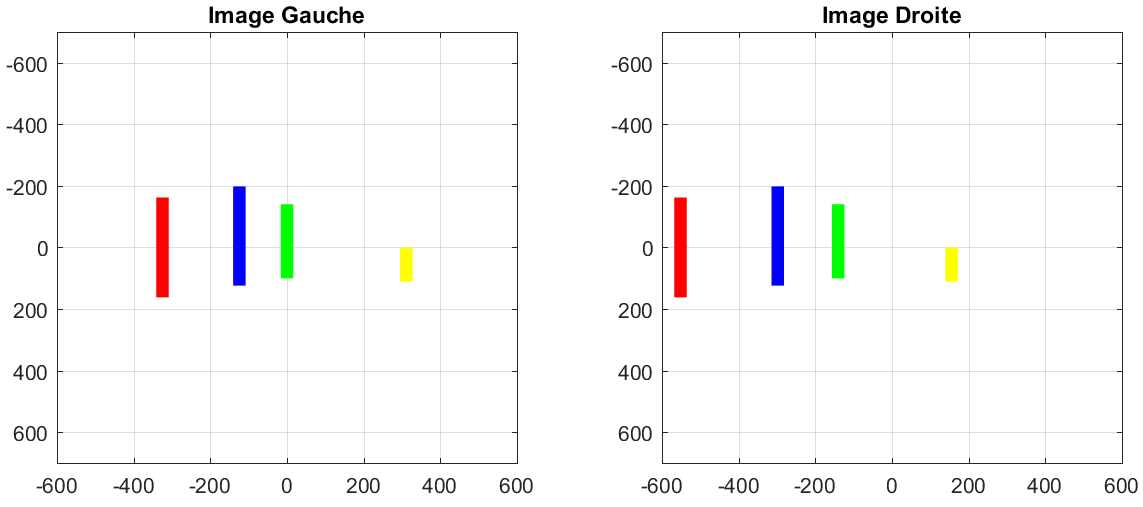
\includegraphics[width=0.95\textwidth]{ImageStereo2.png} 
  \end{tabular}
 \end{center}
\vspace{-0.3in}
 \caption{Paire d'images en stéréo. Les coordonnées sont en pixels.}
 \label{ImageStereo}
\end{figure}


\subsection{Distance focale $f$ (5 pts)}
Estimez la distance focale $f$ (en pixel) de la caméra, en utilisant la tour verte dans l'image de gauche. Donnez le détail de votre calcul.

\subsection{Estimation de la distance $A_z$ de chaque tour (8 pts)}
En mesurant la disparité $d$ entre les centres des tours trouvez leur coordonnée $A_z$ respective. Bien indiquer vos mesures et calculs dans votre rapport, et présentez votre réponse finale dans un tableau comme la Table~\ref{TableCoord}.

\begin{table}[h]
\caption{Distance en $z$ des centres des faces des colonnes.}
\label{TableCoord}
\begin{center}
\begin{tabular}{|c|c|}
\hline
 tour     &    $A_z$ \\
\hline
 rouge      &                          \\
 vert      &                          \\
 bleu      &                            \\
jaune     &                         \\
\hline
\end{tabular}
\end{center}
\end{table}


\subsection{Estimation de la coordonnée $A_x$ de chaque tour (7 pts)}
Retrouvez la coordonnées $A_x$ de chacun des objets par rapport à la caméra de gauche. Faites l'hypothèse que l'axe $X$ de la caméra gauche pointe vers la droite, et que le point principal est situé au centre de l'image. 

\begin{table}[h]
\caption{Coordonnée en $x$ des centres des faces des colonnes.}
\label{TableX}
\begin{center}
\begin{tabular}{|c|c|}
\hline
 tour     &    $A_x$ \\
\hline
 rouge      &                          \\
 vert      &                           \\
 bleu     &                            \\
 jaune     &                         \\
\hline
\end{tabular}
\end{center}
\end{table}

% ==================  FAST =======================
\newpage
\section{Extracteur de coin FAST (15 pts pour GLO-4001, 18 pts pour GLO-7021)}
 \label{SectionFAST}

\subsection{Fonction d'extraction des coins FAST (6 pts)}
Codez une fonction d'extraction de coins basée sur la méthode FAST, pour des cercles tels que montré à la Figure~\ref{FastPixelOrder}. Notez que vous cherchez un coin ayant 12 pixels continus sur l'arc qui satisfassent le critère. La fonction a le prototype suivant :
\vspace{-0.05in}
\begin{minted}{python}
def detection_coin_FAST(image, centre, seuil)
    return is_fast_corner, intensite_coin
\end{minted}
\vspace{-0.05in}
où les arguments en entrée sont :
\begin{itemize}
\item \mcode{image} une image (en noir et blanc);
\item \mcode{centre} un vecteur donnant la coordonnée x-y pour laquelle tester la présence d'un coin dans l'\mcode{image};
\item \mcode{seuil} le seuil $t$, tel que spécifié dans les équations de l'acétate 149 de \texttt{03-VisionII.pdf};
\end{itemize}
et les sorties sont :
\begin{itemize}
\item \mcode{is_fast_corner} indique la présence (1) ou l'absence (0) d'un coin;
\item \mcode{intensite_coin} donne l'intensité du coin représenté par la somme $V$, telle que spécifiée à l'acétate 150;
%\item \mcode{Orientation} donne l'orientation du coin, en radian, basée sur l'acétate 145.
\end{itemize}

\begin{figure}[ht]
 \begin{center}
  \begin{tabular}{c}
    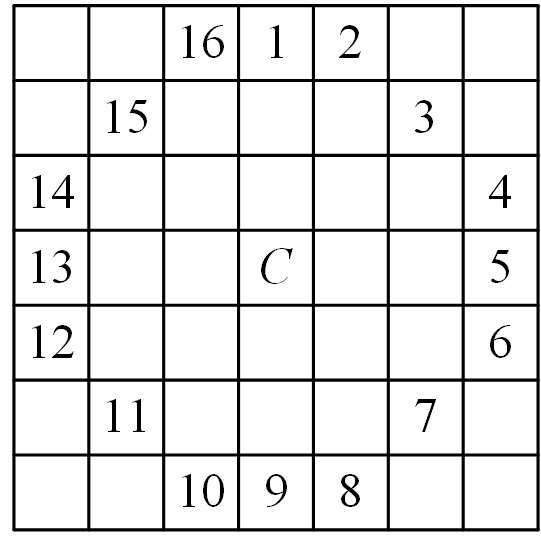
\includegraphics[width=0.25\textwidth]{FastPixelOrder.png} 
  \end{tabular}
 \end{center}
\vspace{-0.25in}
 \caption{Position des pixels à tester pour le détecteur de coin FAST. Les numéros sont à titre indicatif.}
 \label{FastPixelOrder}
\end{figure}

\emph{Bug subtil en matlab! Si vous travaillez avec des UINT8 (ce que fait matlab naturellement pour des images), les valeurs négatives ne seront pas admises! Il vous faudra donc stocker les intensités lumineuses avec des entiers SIGNÉS.}

\subsection{Test de votre fonction \texttt{detection\_coin\_FAST} sur une image réelle (9 pts)}
Vous allez maintenant tester votre détecteur de coin une image réelle, à partir d'un jeu de données qui a été capturé sur l'île de Devon dans l'arctique canadien par un robot mobile de l'équipe du Prof. Barfoot (U. Toronto). Cette île est reconnue mondialement pour sa similarité avec le sol martien, et sert donc souvent de lieu d'essai pour la robotique interplanétaire. L'image en question est \texttt{bw-rectified-left-022148small.png}. Parcourez toute cette image (sauf la bordure à l'intérieur de 8 pixels\footnote{Car il ne sera pas possible d'extraire les features BRIEF de la question suivante pour les bordures.}) et trouvez tous les coins, avec la valeur de \mcode{Seuil} de 10 (voir\footnote{Les intensités dans l'image sont entre 0 et 255, car codé en entier non-signé de 8 bits (\mcode{uint8}).}). Pour chaque coin trouvé, marquez sa position à l'aide d'un petit cercle rouge. Attention! Certaines fonctions d'affichages des images intervertissent les axes x-y.
Répondez aux questions suivantes:
\begin{itemize}
\item Combien de coins trouvez-vous dans cette image? 
\item Quel pourcentage des pixels sont donc considérés comme des coins? 
\item Pourquoi cette scène génère-t-elle ce nombre de coins ? 
\item Quelles régions de l'images contiennent plus de coins? 
\item Moins de coins? 
\end{itemize}
Incluez aussi dans votre rapport l'image avec les coins trouvés.


\subsection{Analyse des résultats (GLO-7021 seulement) (3 pts)}
Afin de limiter le nombre de coins à traiter, il est possible d'utiliser un heuristique simple, qui permet de ne conserver que les coins les plus forts, basé sur la valeur \mcode{intensite_coin}. Cependant, pour utiliser un tel heuristique, il est important de comprendre la distribution de ces valeurs. Dans un histogramme, montrez la distribution des intensités, pour les coins trouvés. Rapportez cette distribution dans votre rapport, et commentez-là.


% ================== Descripteur BRIEF =======================

\newpage
\section{Descripteur BRIEF (19 pts pour GLO-4001, 26 pts pour GLO-7021)}
Le descripteur binaire BRIEF est de plus en plus utilisé pour décrire des points de repères naturels dans des problèmes de localisation par caméra. Cette popularité grandissante est en partie dûe à sa facilité de codage, sa robustesse et sa rapidité de calcul. Dans cette question, vous allez explorer l'utilisation de ces descripteurs BRIEF, extraits autour de coins FAST. Pour vous aider, référez-vous au besoin à l'article original du BRIEF : \url{http://www2.ift.ulaval.ca/~pgiguere/cours/IntroRobotique/notes/calonder_eccv10.pdf} .

\subsection{Fonction calculant un descripteur BRIEF (3 pts)}
En matlab ou python, écrivez une fonction \texttt{ExtractBRIEF(ImagePatch,BriefDescriptorConfig)} qui accepte une patch d'image noir et blanc de SxS pixels avec S=15, ainsi qu'une structure de données \texttt{BriefDescriptorConfig}. Cette fonction retourne le descripteur utilisant \texttt{BriefDescriptorConfig}, dans un format de votre choix. Cette fonction ne devrait être que quelques lignes de code. Plus d'information sur \texttt{BriefDescriptorConfig} est disponible à la question suivante.

\subsection{Pipeline d'extraction de features sur une paire d'images réelles (9 pts pour GLO-4001, 11 pts pour GLO-7021)}
L'extraction de features visuels est en général une opération coûteuse du point de vue calcul. Ainsi, il est préférable de ne se concentrer que sur des points intéressants dans les images, les \emph{keypoints}. À la question~\ref{SectionFAST}, vous avez justement codé une fonction permettant l'extraction de keypoints. Un pipeline d'extraction ressemble typiquement au diagramme de la Figure~\ref{PipelineExtraction}.

\begin{figure}[ht]
 \begin{center}
  \begin{tabular}{c}
    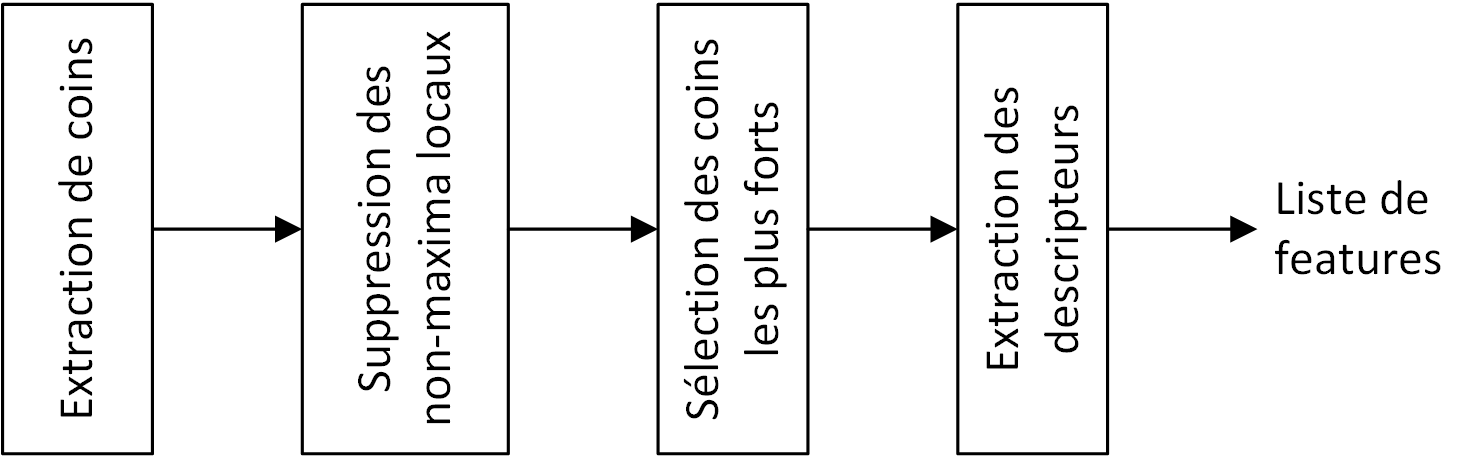
\includegraphics[width=0.6\textwidth]{PipelineExtraction.png} 
  \end{tabular}
 \end{center}
\vspace{-0.25in}
 \caption{Pipeline d'extraction des features, utilisé lors de la recherche de points de repères naturels dans des images.}
 \label{PipelineExtraction}
\end{figure}

Implémentez ce pipeline, en utilisant vos deux fonctions \mcode{detection_coin_FAST} et \mcode{ExtractBRIEF} pour la première et quatrième étape du pipeline. Pour les étudiants en GLO-4001, la suppression des non-maxima locaux est optionnelle. Pour les GLO-7021, implémenter une version approximative de cette suppression, de votre choix. La sélection des coins sera basée sur la valeur de leur intensité \mcode{intensite_coin}: vous ne conserverez que ceux dans le 90ème percentile (autrement dit, les 10~\% les plus forts)\footnote{Une manière facile pour identifier ces coins est de trier la liste des coins selon l'intensité, et de ne conserver que un dixième de cette liste.} . Pour les descripteurs, utilisez \texttt{numberOfBits}=200 bits. Dans ce programme, la structure de données \texttt{BriefDescriptorConfig} qui décrit les \texttt{numberOfBits} paires de pixels testées n'est \underline{initialisée une seule fois}. Pour générer ces paires de pixels (obligatoirement de manière aléatoire), utilisez une distribution uniforme (\texttt{rand()}) sur SxS, avec S=15. Ne vous préoccupez pas des doublons possibles sur ces paires de pixels, pour vous sauver du temps de codage. Assurez-vous que ces paires sont des entiers, via la fonction \texttt{ceil()}. Le descripteur doit être extrait dans une fenêtre centrée sur le coin FAST.

Pour les étudiants en GLO-7021, commentez sur :
\begin{itemize}
\item votre stratégie pour la suppression des non-maxima locaux;
\item le pourcentage des coins retirés
\end{itemize}

\subsection{Appariement features image gauche-droite (7 pts)}
 Appliquez votre pipeline sur les images suivantes :
 \begin{itemize}
 \item \texttt{bw-rectified-left-022148small.png} et
 \item \texttt{bw-rectified-right-022148small.png}, 
 \end{itemize}
 disponibles dans le répertoire inclus avec ce TP. Ces images sont issues d'une caméra stéréo. Pour chaque descripteur de l'image de gauche, trouvez le feature dans l'image de droite qui a la plus petite distance de Hamming, donc le plus semblable. Ceci constituera l'appariement. Dans dans votre rapport, mettez une image représentant ces matches. Le fond sera l'image de gauche, et chaque ligne verte reliera le feature de gauche au feature de droite associé, comme dans l'image~\ref{ExempleImageMontrantMatches}. Si vous avez trop de lignes, choisissez-en un nombre raisonnable de manière aléatoire (une centaine) pour affichage.

\begin{figure}[ht]
 \begin{center}
  \begin{tabular}{c}
    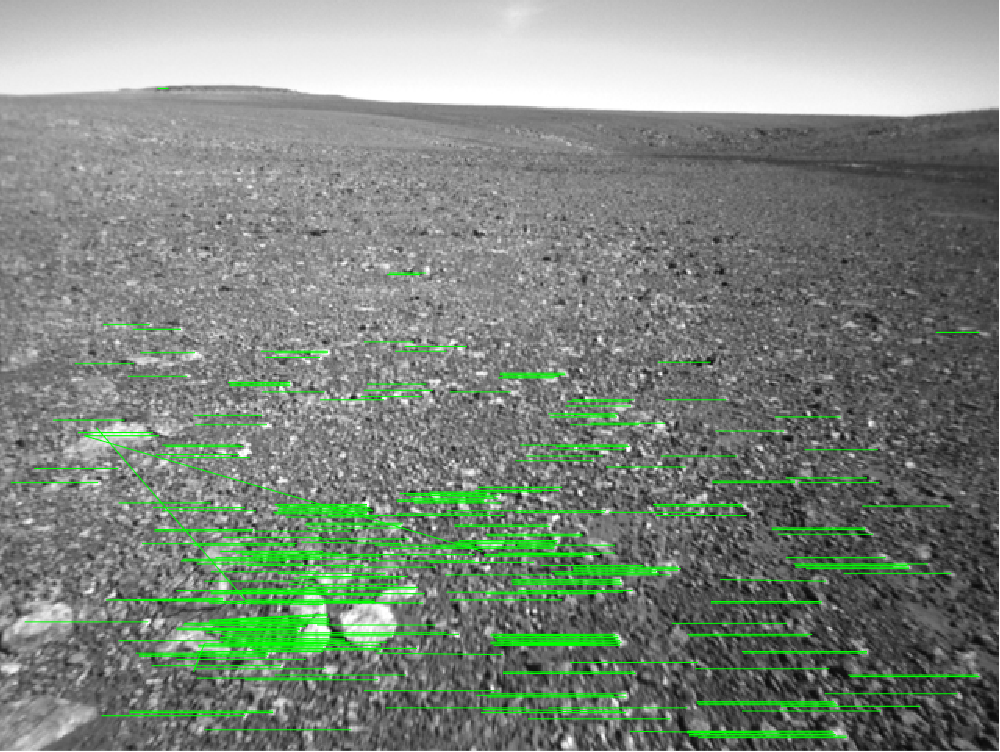
\includegraphics[width=0.75\textwidth]{ExempleImageMontrantMatches.png} 
  \end{tabular}
 \end{center}
\vspace{-0.25in}
 \caption{Image similaire à celle que vous devez utiliser, et montrant quelques appariements entre les features de l'image gauche (en fond) vers les features de l'image droite. Notez que j'ai épuré ces matches, afin de ne conserver que de très bons. Vous devriez avoir plus de lignes diagonales dans votre résultat.}
 \label{ExempleImageMontrantMatches}
\end{figure}

\subsection{Amélioration de la qualité des matchs (GLO-7021 Seulement) (7 pts)}
Vous devriez constater que vous avez beaucoup de faux matches dans l'image. Tentez d'améliorer la qualité de ces matches, en utilisant deux stratégies, soit celles vues en classe, soit de votre crue. Commentez sur l'amélioration apportée par chacune de vos stratégies.


% ================== CAMERA =======================
\newpage
\section{Modèle de caméra et positionnement par caméra (26 pts pour GLO-4001, 36 pts pour GLO-7021)}
Ces exercices serviront à vous familiariser à la fois au processus de génération d'images et de localisation par caméra, ainsi qu'aux concepts de matrices intrinsèques/extrinsèques de caméra. Dans un premier temps, vous aller devoir faire le code permettant la génération d'images pour un monde simplifié. Dans un deuxième temps, vous allez utiliser du code pour vous localiser par minimisation d'erreur de reprojection. Finalement, à l'aide de nombreuses simulations, vous allez être à même de voir l'impact de plusieurs paramètres du problème (position de la caméra, position des repères, nombre de repères) sur l'incertitude de la relocalisation. 

\subsection{Génération d'une image (6 pts)}
Vous avez trois points de repère, situé au coordonnées \emph{globales} suivantes (en $m$):
\begin{itemize}
\item $L_1$ : [-0.2, 0 , 1.2]
\item $L_2$ : [ 0, \hspace{0.08in} 0   , 1]
\item $L_3$ : [0.2, \hspace{0.03in} 0, 1.2]
\end{itemize}
Pour le repère global, l'axe des $y$ pointe en s'éloignant de vous. L'axe des $x$ pointe vers la droite et l'axe des $z$ vers le haut. Le tout est illustré à la Figure~\ref{DiagLocalisation}. Vous allez avoir une caméra dont l'axe optique est parallèle au plancher, et l'axe des $y$ pointe vers le bas (comme pour le repère global). La distance focale de la caméra est de $f=1000$ pixels.

\begin{figure}[ht]
 \begin{center}
  \begin{tabular}{c}
    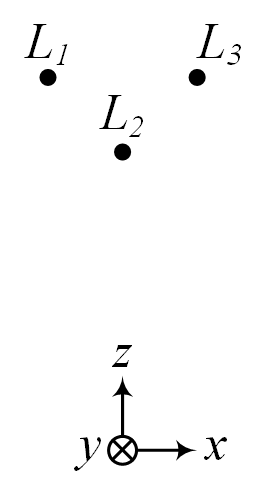
\includegraphics[width=0.15\textwidth]{LocalisationCamera.png} 
  \end{tabular}
 \end{center}
\vspace{-0.3in}
 \caption{Diagramme illustrant la position des points de repères par rapport au repère global.}
 \label{DiagLocalisation}
\end{figure}

En Python, faites une fonction \texttt{reprojection()} qui prend la photo :
\vspace{-0.05in}
\begin{minted}{python}
def reprojection(H, focale, L):
\end{minted}
\vspace{-0.05in}
c'est-à-dire qui calcule la positions des trois points de repère $L_i$ dans les coordonnées $u$ et $v$ du plan image de la caméra. Cette fonction accepte aussi la focale de la caméra et la pose \texttt{H} de la caméra dans le repère globale, exprimée par une matrice de transformation homogène 4x4.
Notez que selon la convention choisie, l'axe $v$ du plan image pointe vers le bas et l'axe $u$ vers la droite. Incluez dans votre rapport les coordonnées images obtenues.

Pour faciliter la lecture de votre code (et pour vous-même), utilisez des Numpy arrays et l'opérateur de multiplication de matrice \texttt{@} dans cette fonction.
{\bf Attention!} La matrice \texttt{H} est la pose de la caméra, exprimée dans le repère global. Ce n'est donc pas la matrice extrinsèque. Cette dernière devra donc être calculée par vous.

En plaçant la caméra à l'origine (donc, l'axe optique de la caméra pointe dans la même direction que l'axe des $z$), prenez une photo. Rapportez les coordonnées dans l'images des trois points de repères $L_i$ dans votre rapport, et sauvegarder ces valeurs dans \texttt{C}, qui deviendra votre image, dite \emph{cible}, pour la question suivante.

\subsection{Localisation par minimisation de l'erreur de reprojection (9 pts)}
Une manière de pouvoir vous localiser à l'aide d'une caméra consiste à minimiser l'erreur de reprojection, qui se basera sans grande surprise sur la fonction  \texttt{reprojection()}. La pose de la caméra minimisant l'écart entre les points de repères dans l'image cible \texttt{C} et ceux calculés par la fonction de reprojection sera considérée comme la bonne. Pour trouver cette pose, vous allez devoir utiliser la fonction d'optimisation \texttt{fmin}\footnote{\url{https://docs.scipy.org/doc/scipy/reference/generated/scipy.optimize.fmin.html}}:
\begin{minted}{python}
from scipy.optimize import fmin
\end{minted}
Pour simplifier le tout, nous allons aussi faires des hypothèses simplificatrices. Ainsi, la caméra ne pourra se déplacer qu'en trois degrés de libertés seulement. Conséquemment, les seuls paramètres de la pose de la caméra qui seront optimisés par \texttt{fmin} lors de la recherche de la pose seront les suivants:
\begin{itemize}
    \item la position en $x$;
    \item la position en $z$; et
    \item l'angle $\theta$ de rotation (autour de l'axe $y$). Un angle $\theta=0$ signifiera que l'axe optique est parallèle à l'axe des $z$ du repère global.
\end{itemize}
La localisation consistera donc à résoudre la minimisation de l'erreur de reprojection au carré pour tous les points de repères $L_i$.
L'erreur de reprojection (dit \emph{résiduel}) $r_i$, pour un point de repère $L_i$ imagé est la distance euclidienne suivante :
\begin{equation}
r_i= || c_i-f_{reprojection}(L_i)||,
\end{equation}
où $c_i$ représente la position (en pixel) du repère $i$ dans l'image cible. Notez que la fonction $f_{reprojection}$ dépendra des paramètres intrinsèques et extrinsèques de la caméra, que j'ai omis ci-haut pour alléger la notation.
La recherche de la pose de la caméra sera donc la minimisation suivante :
\begin{equation}
    \argmin_{x,y,\theta} \sum_{i \in Repere} r_i^2.
\end{equation}


%Votre travail consistera donc à:
%\begin{itemize}
%    \item bien calculer la matrice extrinsèque $\mathbf{M}$ dans la fonction de reprojection, pour exprimer les points $\mathbf{p}$ dans le référentiel de la caméra. Notez que cette matrice $\mathbf{M}$, calculée à partir de $\mathbf{H}$, changera à chaque itération (car $\mathbf{H}$ lui-même changera, en fonction de la pose actuelle dans l'optimiseur).

La fonction à minimiser (à implémenter) sera :
\begin{minted}{python}
def somme_des_residuels_au_carre(pose_camera,focal,L,C):
\end{minted}
où \texttt{pose\_camera} sera un vecteur contenant les valeurs $[x,z,\theta]$ de la pose de la caméra, exprimé dans le repère monde,
\texttt{C} contient les coordonnées de tous les repères $\mathbf{L}$ dans l'image cible, \texttt{L} contiendra les coordonnées 3D en homogènes des points de repères dans le repère global, et \texttt{focale} sera la focale de la caméra.

L'optimisation se fera avec la commande suivante :
\begin{minted}{python}
pose_solution = fmin(somme_des_residuels_au_carre, pose_initiale_camera, 
                      args=(focal, L, C), maxiter=1000)
\end{minted}
La \texttt{pose\_initiale\_camera} sera un vecteur contenant les valeurs estimées $[x,z,\theta]$ de la pose de la caméra. Notez ici qu'ils correspondent aussi aux variables libres dans l'optimisation. Dans votre cas, initialisez ce vecteur à un endroit légèrement décalé de la position réelle, soit d'environ 0.2 unités pour $x$ et $z$ et d'environ 0.2 rad pour $\theta$.
Dans votre rapport, indiquez:
\begin{itemize}
    \item le nombre d'itérations effectués par \texttt{fmin};
    \item la solution trouvée et son écart par rapport à la vraie pose $[x,z,\theta]= [0, 0, 0] $.
\end{itemize}

\subsection{Impact du bruit sur l'estimation des repères via une approche de type Monte Carlo (10 pts pour GLO-4001, 7 pts pour GLO-7021)}
\label{sec:ImpactBruit}
En réalité, la détection de point de repères dans une image ne se fait pas parfaitement. Ainsi, il y aura une petite erreur entre la position estimée et la position réelle, en pixel, de ces repères. Vous allez simuler cela en ajoutant du bruit sur la coordonnée en $u$ de ces repères. Nous n'ajoutons pas de bruit en $v$ car nous ne sommes intéressés que par la position horizontale de ces repères dans l'image. Ce bruit suivra une distribution gaussienne, avec écart-type $\sigma_p=2$~pixel.

Montrez la distribution des estimés de pose de la caméra sur une carte 2D $(x,z)$, en traçant un point par estimé trouvé par simulation. Chaque simulation consiste simplement à piger les bruits aléatoirement, de les additionner au valeurs véritables des $u$, puis de retrouver la pose avec la méthode de la section précédente. Répétez cette routine mais pour des nouvelles poses de caméras en la reculant de 1 à 7~$m$, par incrément de 1~$m$.

Pour chaque pose, faites 1000 simulations bruitées et marquez d'un point sur un graphique la pose trouvée, afin de visualiser approximativement cette distribution. Par exemple, la Figure~\ref{ExampleDistribution} montre un ensemble hypothétique de distributions illustrées de la manière demandée, pour des poses (entre 0 et 7~$m$) comparables à l'exercice demandé.

\begin{figure}[ht]
 \begin{center}
  \begin{tabular}{c}
    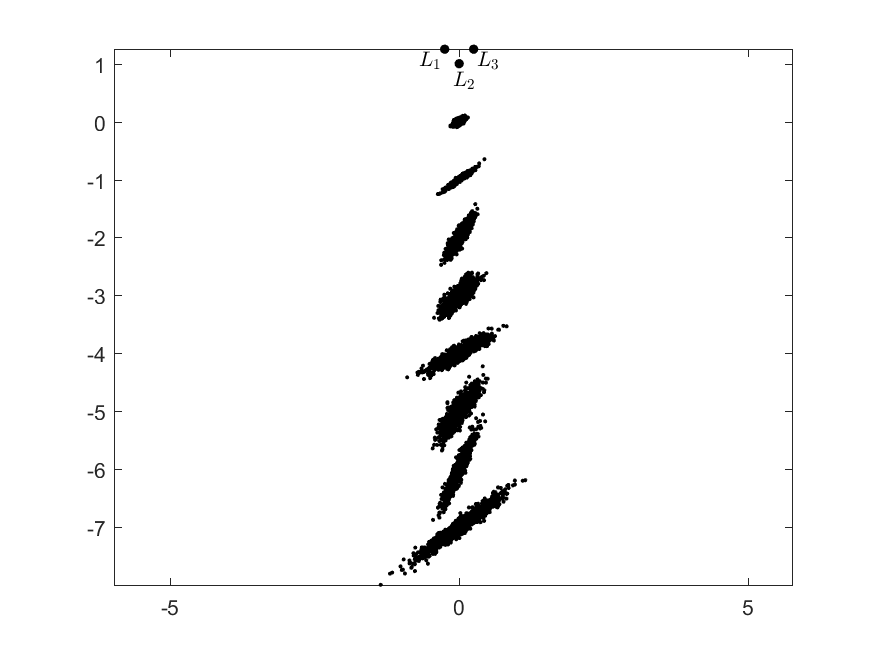
\includegraphics[width=0.65\textwidth]{ExampleDistribution.png} 
  \end{tabular}
 \end{center}
\vspace{-0.3in}
 \caption{Exemple de distributions quelconques (non, ce n'est pas la solution!) pour différentes poses de la caméra. Notez la position fixe des repères $L_i$, tel que demandé dans l'exercice, et le centre des distributions qui reculent, selon $z_{carte}$.}
 \label{ExampleDistribution}
\end{figure}


\subsection{Discussion sur la forme de la distribution  (3 pts) GLO-7021 seulement}
\label{sec:FormeDistr}

Calculez la covariance empirique de cette distribution pour chacune des poses. Que remarquez-vous sur la forme de ces distributions, en particulier les termes en dehors de la diagonale de cette matrice de covariance ? À quoi attribuez-vous cela ?

Tracez une figure montrant les écart-types $\sigma_{xcarte}$ et  $\sigma_{ycarte}$, en fonction des huit poses réelles (de 0 à 7~$m$). Discutez.

\subsection{Influence de la position des points de repère sur la qualité de la localisation (3 pts) GLO-7021 seulement}
Doublez l'espacement des points de repère, tout en conservant la même position pour $L_2$ et la même configuration (en triangle) des trois points de repères. Refaites les expériences des sections \ref{sec:ImpactBruit} et \ref{sec:FormeDistr}. Commentez sur l'impact de l'incertitude de localisation, en fonction de cette augmentation de la distance entre les repères.

\subsection{Influence du nombre de points de repère sur la qualité de la localisation  (7 pts) GLO-7021 seulement}
Une règle de base que l'on a vu en classe est que l'incertitude d'un estimé diminue généralement en $1/\sqrt{n}$, où $n$ est le nombre de mesures utilisées. En dispersant aléatoirement $n$ points de repères devant la caméra en suivant une distribution normale entre -0.5 et 1.5~$m$ en $z$ et -0.5 et 0.5~$m$ en $x$, estimez la précision de la localisation. Réutilisez votre code de la question \ref{sec:ImpactBruit}. 

Commentez en un paragraphe l'impact du nombre de points de repères $n$ sur l'incertitude de localisation. Justifiez le choix des $n$ dans votre expérimentation. Ajoutez des graphiques montrant l'écart type en $x$ et en $z$ de la localisation, en fonction de $n$.


\end{document}
